\section{Case Studies}%
\label{sec:eval.studies}

In this section, we aim to demonstrate our solution when applied to four
different case studies, each presenting a parametric geometric shape: an egg, a
rounded trapezoid, a star with semicircles, and a Voronoi diagram.  Each case,
illustrated in \cref{fig:eval.studies.designs}, was inspired by an existing
design:
\begin{enumerate*}[label= (\arabic*)]
  \item Eero Aarnio's Egg chair, 
  \item Thonet 214 chair seat,
  \item César Pelli's Petronas tower section, and
  \item PTW Architects' Beijing National Aquatics Center.
\end{enumerate*}
These cases present a set of \ac{GC} problems involving circles and lines, such
as \textit{tangent line to two circles} and \textit{circle-line intersection}.
These problems were solved employing both an \textit{analytic} approach, an
approach \acp{TPL} naturally demand, and a \textit{constructive} approach, the
one made possible by relying on our solution.

\begin{figure}[htb]
  \subcaptionbox{Egg chair.\label{fig:eval.studies.designs.egg}}
    [.2\linewidth]{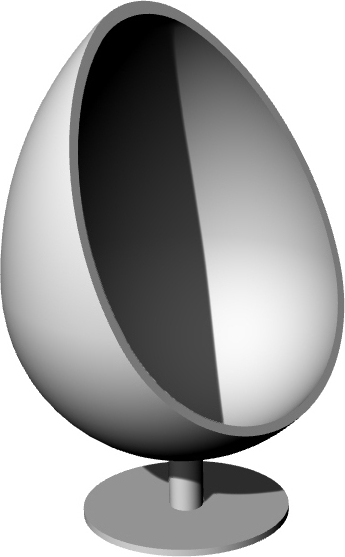
\includegraphics[height=4cm]{fig/case-study-egg-chair}}
  \hfill
  \subcaptionbox{Simple 4-leg chair.\label{fig:eval.studies.designs.thonet214}}
    [.2\linewidth]{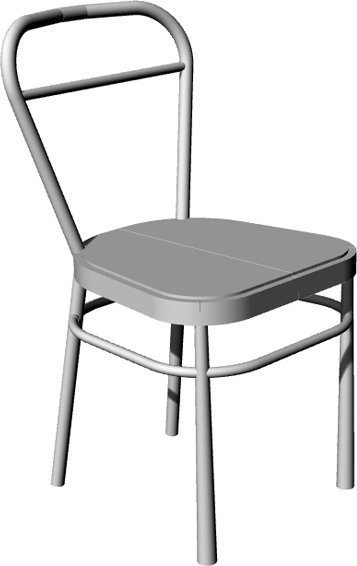
\includegraphics[height=4cm]{fig/case-study-thonet-214}}
  \hfill
  \subcaptionbox{Islamic towers.\label{fig:eval.studies.designs.petronas}}
    [.2\linewidth]{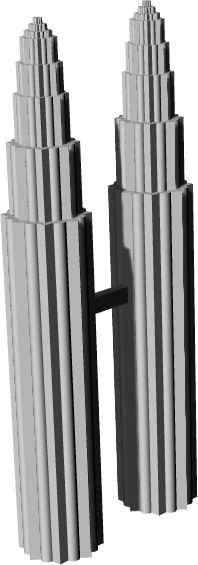
\includegraphics[height=4cm]{fig/case-study-petronas}}
  \hfill
  \subcaptionbox{Voronoi cage.\label{fig:eval.studies.designs.watercube}}
    [.35\linewidth]{%
      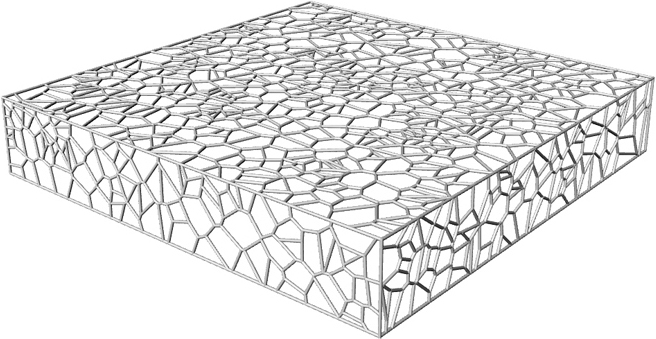
\includegraphics[width=\linewidth]{fig/case-study-water-cube}}
  \caption[Case study design inspirations]{
    Case study designs inspired by the Eero Aarnio's Egg
    chair~\subref{fig:eval.studies.designs.egg}, Thonet 214
    chair~\subref{fig:eval.studies.designs.thonet214},  César Pelli's Petronas
    Twin Towers~\subref{fig:eval.studies.designs.petronas}, and PTW Architects'
    Beijing National Aquatics
    Center~\subref{fig:eval.studies.designs.watercube}.}%
  \label{fig:eval.studies.designs}
\end{figure}

\subsection{Egg}%
\label{sec:eval.studies.egg}

The first case study is an egg shape (which can be considered a particular case
of an oval shape).  Examples of applications of this shape in design include the
Eero Aarnio's Egg chair, James Law's Cybertecture Egg building, and RAU
Architects and Ro\&Ad Architects' Tij observatory.

The egg shape is a broad concept, as it can refer to a wide range of curves
resembling an egg~\cite{Dixon:1991:Mathographics}.  In this case, our shape is
bilaterally symmetric and is composed of four arcs, the side arcs being tangent
to the bottom and top arcs.

Our parametrization of the egg defines four parameters: the bottom arc's center
$O_1$, the bottom and top arcs' radii $r_1$ and $r_2$ respectively, and the
egg's height $h$ (\cref{fig:eval.studies.egg.prob.params}).  Different egg
shapes, more or less elongated, can be obtained by varying the parameters'
values (\cref{fig:eval.studies.egg.prob.vars}).  One of those variations, where
$r_2 = (2 - \sqrt2)r_1$ and $h = 2r_1 + r_2$, corresponds to the Moss' Egg
(\cref{fig:eval.studies.egg.prob}, the egg with $h = 2.6$ and $r_2 = 0.6$).

\begin{figure}[htb]
  \subcaptionbox{\label{fig:eval.studies.egg.prob.params}%
    Egg parametrization: center $O_1$, bottom and top arcs' radii $r_1$ and
    $r_2$, and height $h$.}
    {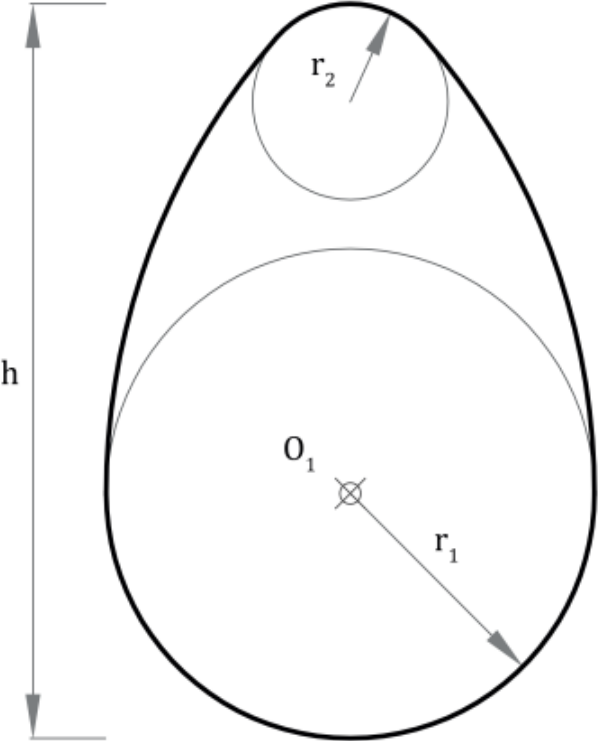
\includegraphics[height=7cm]{fig/egg-problem-params}}
  \hfill
  \subcaptionbox{\label{fig:eval.studies.egg.prob.vars}%
    Egg shape variations: variations change the values of the radius $r_3$ and
    the height $h$.}
    {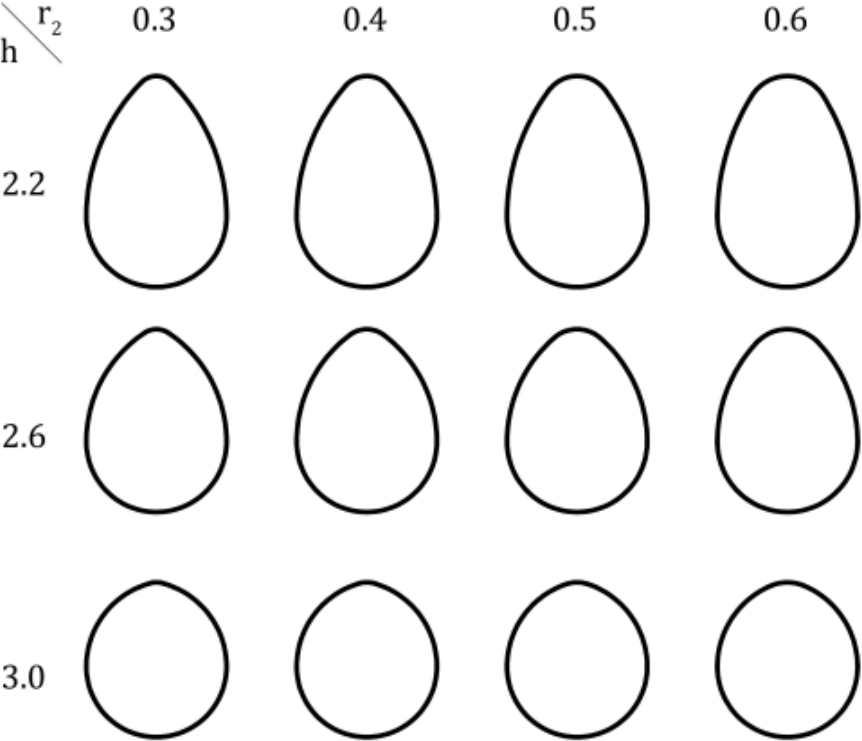
\includegraphics[height=7cm]{fig/egg-problem-vars}}
  \caption[Egg problem]{Egg problem:
  \subref{fig:eval.studies.egg.prob.params} shows our parametrization of the
  egg which can be used to generate shape variations, some of them shown in
  \subref{fig:eval.studies.egg.prob.vars}.}\label{fig:eval.studies.egg.prob}
\end{figure}

In this case, the major problem was to define the side arc $A_3$, which is given
by the center $O_3$, radius $r_3$, and amplitude $\alpha$
(\cref{fig:eval.studies.egg.sol.a}). The \textit{analytic solution} is described
below. The angle $\alpha$ and the radius $r_3$ are devised from the triangle
$\triangle O_1 O_2 O_3$ (\cref{fig:eval.studies.egg.sol.c}), and the center
$O_3$ is given by a translation of $O_1$ through the unit vector $\vec{e}_x$,
parallel to the X-axis, scaled by the factor $r_1 - r_3$.  It is important to
note that, despite their simplicity, the derivations needed to arrive at the
following formulas are not obvious.

\begin{enumerate}
  \item $\alpha = 2\arctan\frac{r_1 - r_2}{h - r_1 - r_2}$
  \item $r_3 = \frac{r_1 - r_2 \cos\alpha}{1 - \cos\alpha}$
  \item $O_3 = O_1 + \left(r_1 - r_2\right)\vec{e}_x$
\end{enumerate}

The \textit{constructive solution} is based on the geometric problem of
determining the \textit{tangent line to two circles}.  In fact, the side arc
$A_3$ is tangent to two circles, $C_1$ and $C_2$, and passes through point
$P_1$.  Two \ac{GC} primitives from our solution were employed in this
solution, namely \textit{intersection} and \textit{bisector}.  The solution can
be computed according to the following procedure
(\cref{fig:eval.studies.egg.sol.c}):

\begin{enumerate}
  \item $C_{2}' = \mathrm{circle}\left(P_1, r_2\right)$%
  \label{enum:eval.studies.egg.cs}
  \item $I = \mathrm{intersection}\left(C_{2}', \overline{O_1 P_2}\right)$
  \item $B = \mathrm{bisector}\left(\overline{IO_2}\right)$
  \item $O_3 = \mathrm{intersection}\left(B, O_1 P_1\right)$
  \item $r_3 = \mathrm{length}\left(\overline{O_3 P_1}\right)$%
  \label{enum:eval.studies.egg.ce}
  \item $\alpha = \mathrm{angle}\left(O_2,O_3,O_1\right)$
\end{enumerate}

We can further increase the expressive level of the solution by defining the
$\mathrm{tangent_{circle}}$ functionality.  Given two circles, $C_1$ and $C_2$,
and a point $P_1$ on $C_1$, $\mathrm{tangent_{circle}}$ produces the circle
tangent to both $C_1$ and $C_2$ that goes through $P_1$.  This way, the solution
can be simplified by replacing steps \ref{enum:eval.studies.egg.cs} through
\ref{enum:eval.studies.egg.ce} by using the $\mathrm{tangent_{circle}}$
functionality as follows:

\begin{enumerate}
  \item $O_3,r_3 = \mathrm{tangent_{circles}}\left(C_1, C_2, P_2\right)$
  \item $\alpha = \mathrm{angle}\left(O_2, O_3, O_1\right)$
\end{enumerate}

In the egg's case, $C_1$ must be larger than $C_2$, and $P_1$ is one of the
intersection points between the horizontal line that passes through $O_1$ and
the circle $C_1$.

\begin{figure}[htb]
  \subcaptionbox{\label{fig:eval.studies.egg.sol.a}%
      Solution using the analytic approach.}
    {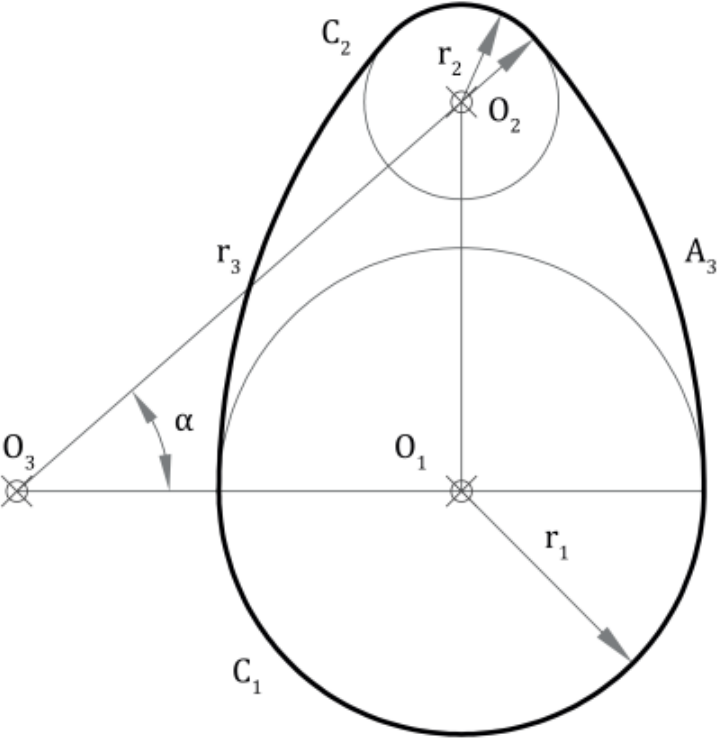
\includegraphics[height=7cm]{fig/egg-solution-analytic}}
  \hspace{\fill}
  \subcaptionbox{\label{fig:eval.studies.egg.sol.c}%
      Solution using the constructive approach.}
    {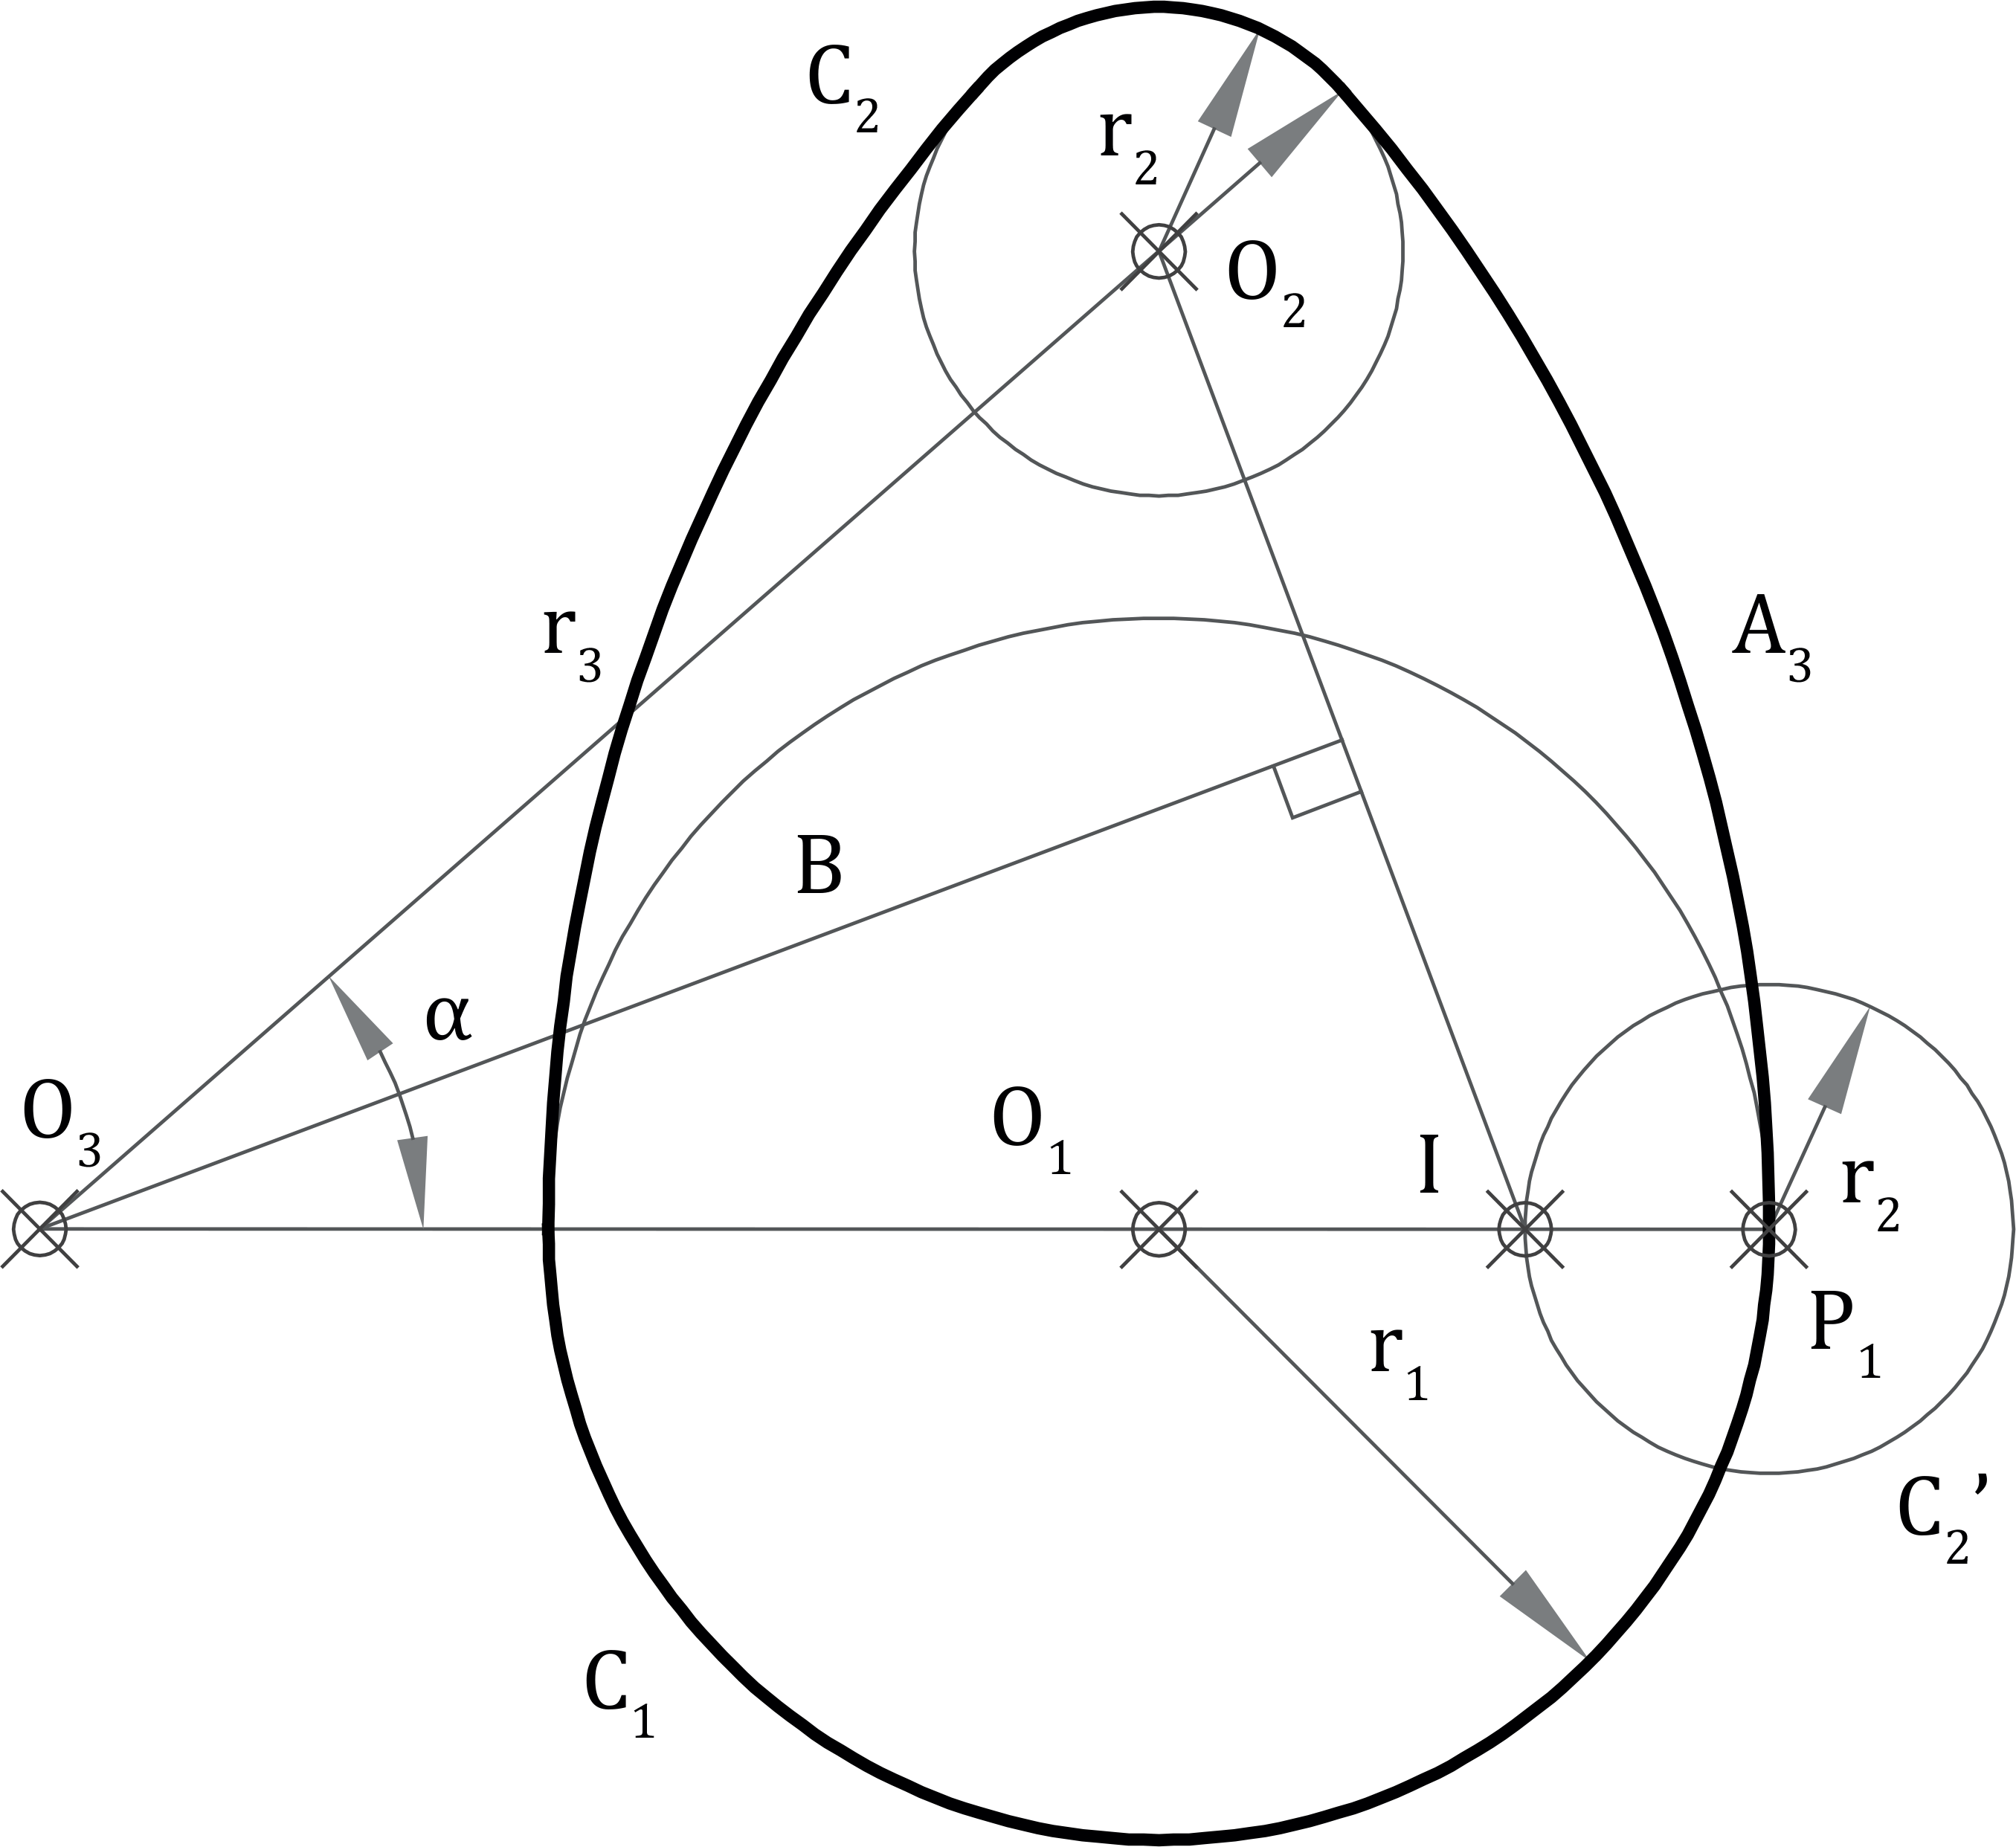
\includegraphics[height=7cm]{fig/egg-solution-constructive}}
  \caption[Egg problem solutions]{Solutions to the Egg problem using two
    different approaches.}%
  \label{fig:eval.studies.egg.sol}
\end{figure}

Achieving the equations in the \textit{analytic solution} is not a
straightforward task for designers, since it involves considerable logical
reasoning and the use of non-trivial formulas (such as trigonometric half-angle
identities). It is also unclear how those equations were derived. By contrast,
in the \textit{constructive solution}, all the steps are clearly externalized,
which makes it much more comprehensible.

\subsection{Rounded Trapezoid}%
\label{sec:eval.studies.rtrapezoid}

The second case study is a rounded trapezoid shape.  This parametric shapes is
used in the contour of a variety of different chair seats, such as the Thonet
214 and the Zig Zag chairs~\cite{Garcia:2018:SGDTIMCG}.  This shape is
bilaterally symmetric and is defined by six parameters: width $w$, depth $d$,
taper width $tw$, front radius $r_f$, rear radius $r_r$, and origin $O$
(\cref{fig:eval.studies.rtrapezoid.prob.params}).  The taper width and front and
rear radii are ratios of the width and the depth.  By varying these parameters'
values, one can obtain different shapes, such as a square, a trapezoid, a
triangle, a rounded rectangle, a drop-like shape, and a circle, among others
(\cref{fig:eval.studies.rtrapezoid.prob.vars}).

\begin{figure}[htb]
  \subcaptionbox{\label{fig:eval.studies.rtrapezoid.prob.params}%
    Trapezoid parametrization: width $w$, depth $d$, taper width $w$, front and
    rear radii $r_f$ and $r_r$ respectively, and origin $O$.}
    {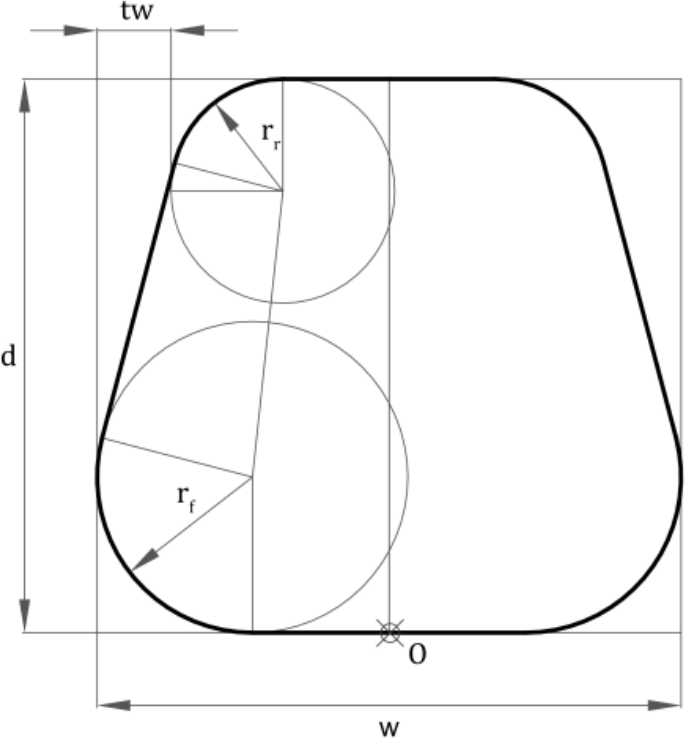
\includegraphics[height=7cm]{fig/rtrapezoid-problem-params}}
  \hfill
  \subcaptionbox{\label{fig:eval.studies.rtrapezoid.prob.vars}%
    Rounded trapezoid shape variations: variations change the values of the
    front radius $r_f$ and the taper width $tw$.}
    {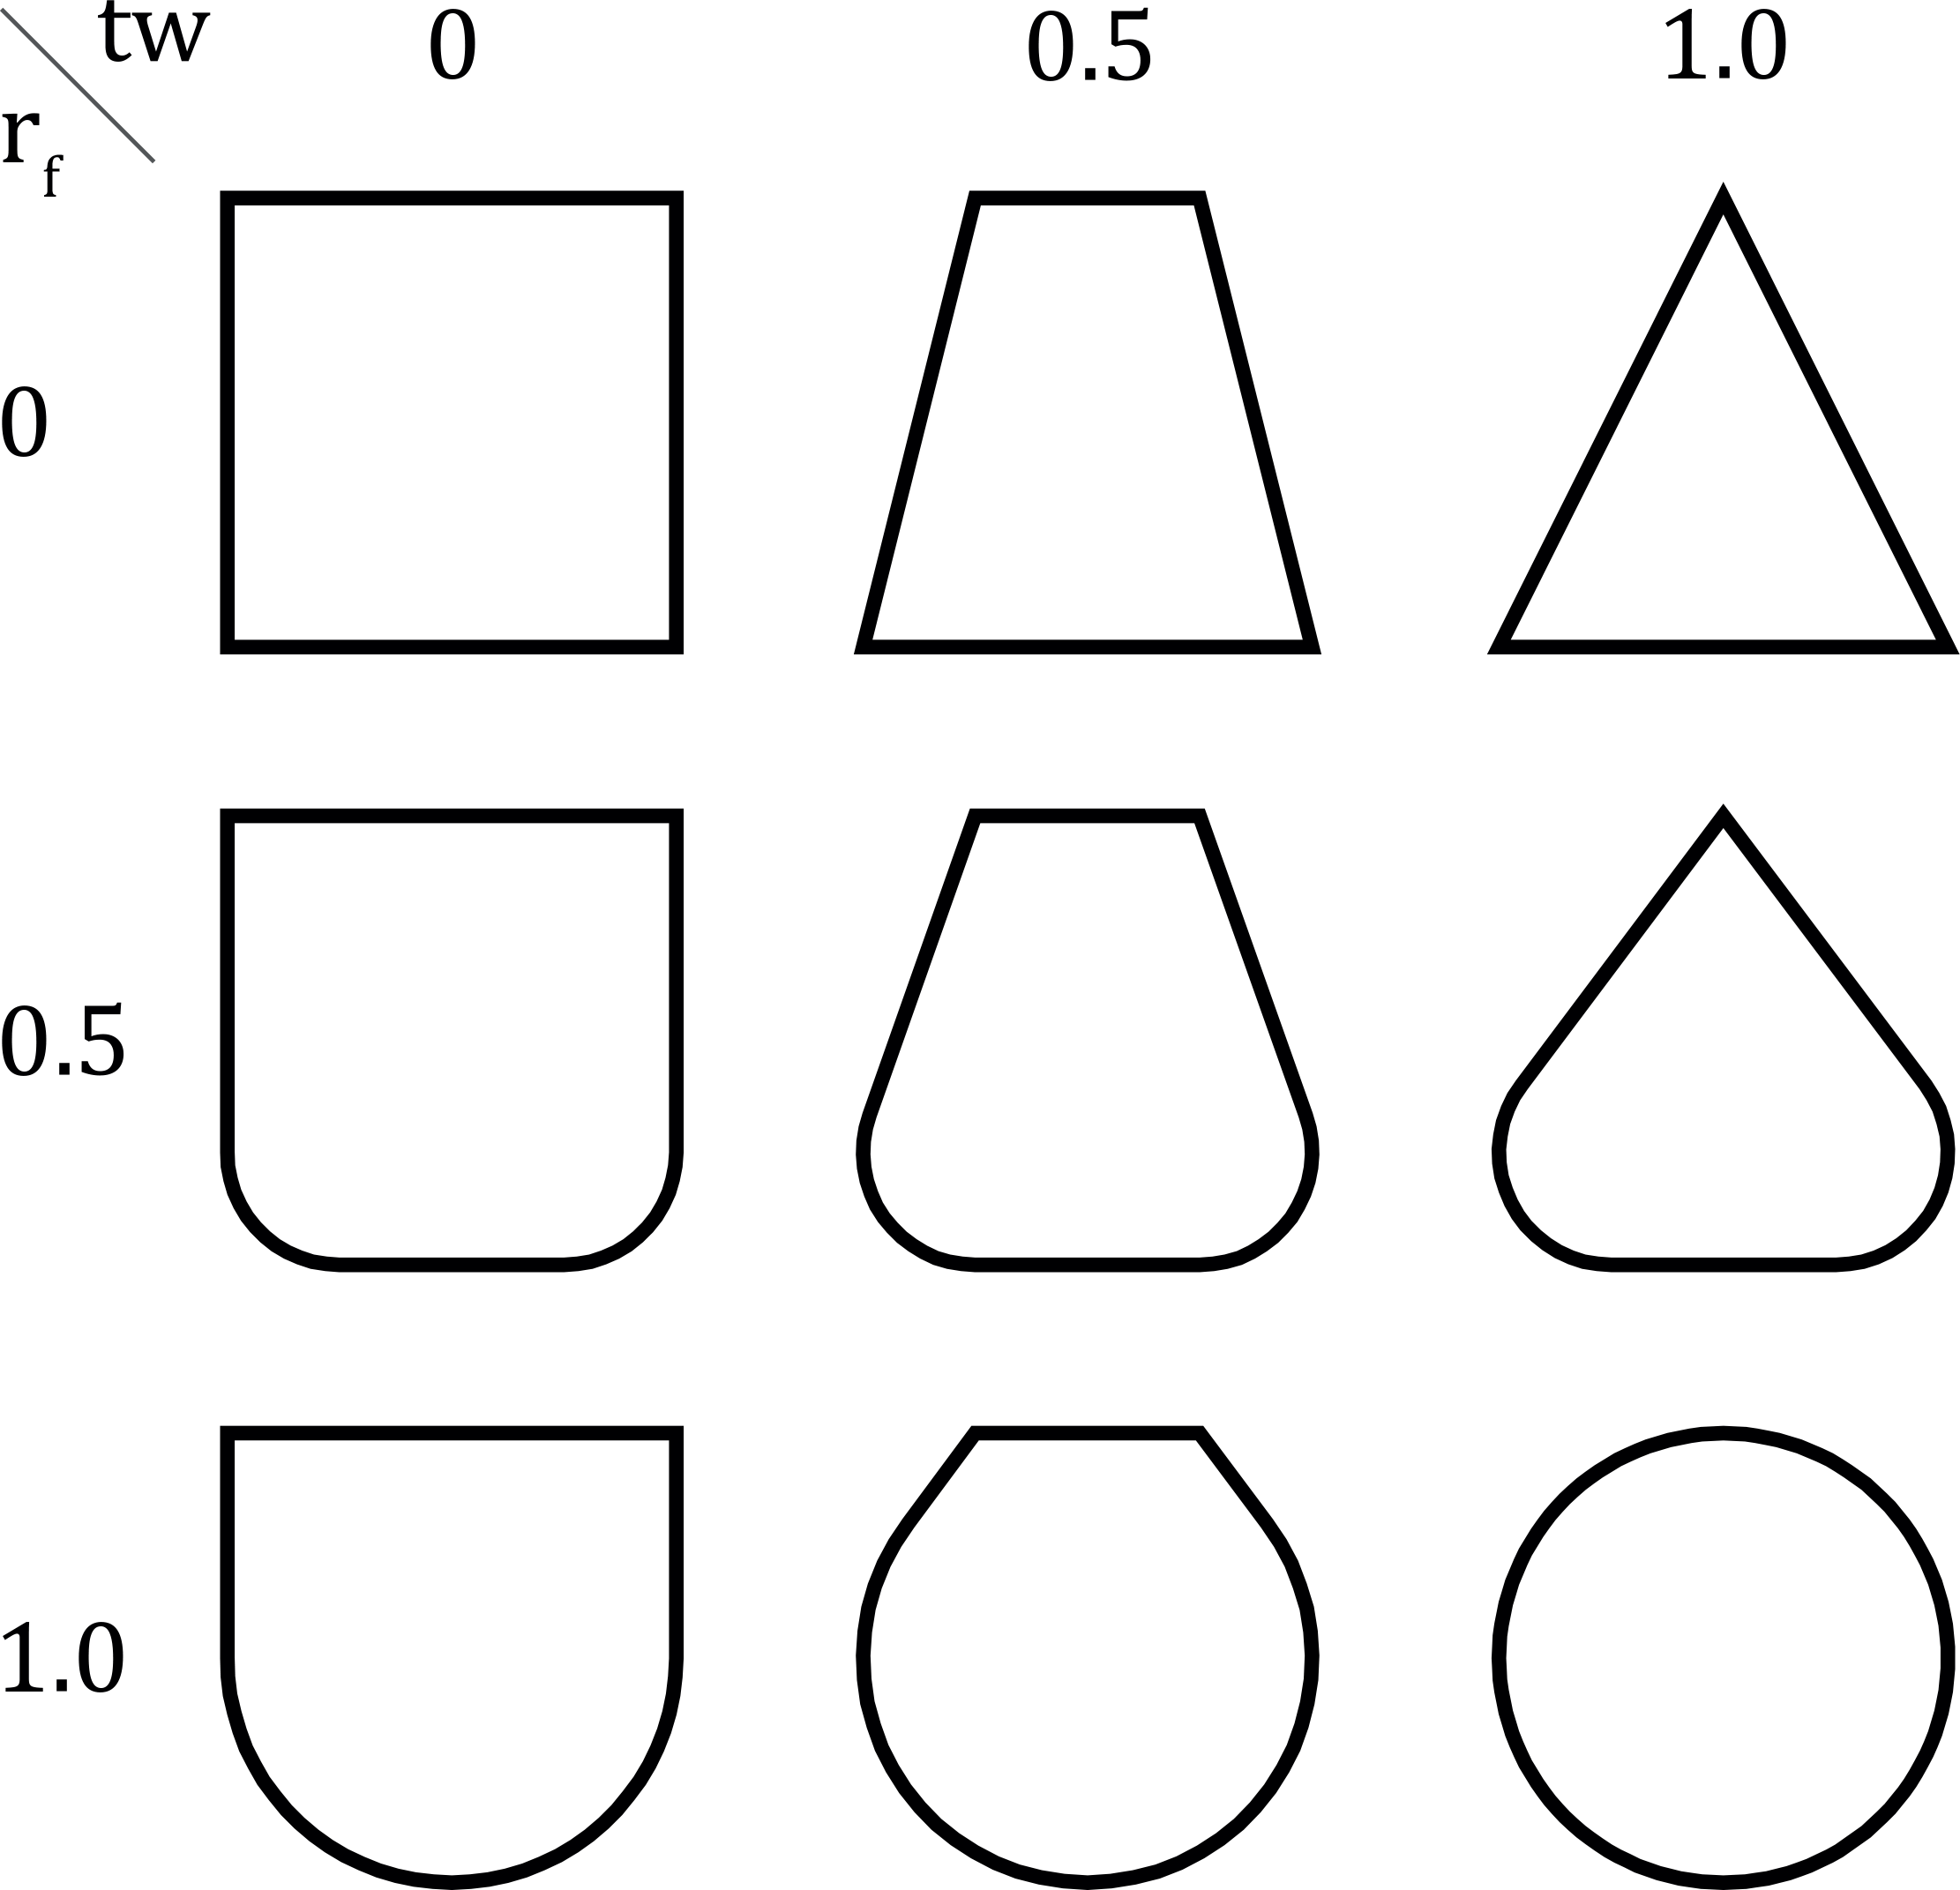
\includegraphics[height=7cm]{fig/rtrapezoid-problem-vars}}
  \caption[Rounded trapezoid problem]{Rounded trapezoid problem:
    \subref{fig:eval.studies.rtrapezoid.prob.params} shows our parametrization
    of the trapezoid which can be used to generate shape variations, some of
    them shown in \subref{fig:eval.studies.rtrapezoid.prob.vars}.}%
  \label{fig:eval.studies.rtrapezoid.prob}
\end{figure}

One side of the chair is obtained by two circles and the \textit{tangent line to
two circles}, while the other side is a reflection of the former side.  Given
two circles $C_2$ and $C_2$, centered on $O_1$ and $O_2$ with radii $r_1$ and
$r_2$ respectively (\cref{fig:eval.studies.rtrapezoid.sol}), two solutions can
be delineated that can accurately reproduce the tangent line $\overline{T_1
T_2}$.

The \textit{analytic solution} is achieved by calculating the angle $\delta$
between the line segment $\overline{O_1 O_2}$ and the line perpendicular to the
tangent line between the two circles passing through $O_1$.  The angle $\theta$
is given by the slope of $\overline{O_1 O_2}$.  The point $T_1$ is given by a
translation of $O_1$ through a vector $\left(r_1, \angle\delta + \theta\right)$
where $r_1$ is its length and $\angle\delta + \theta$ is its polar angle.  A
similar approach is used to obtain $T_2$.

\begin{enumerate}
  \item $\delta = \arccos\frac{r_1 - r_2}{\lVert O_2 - O_1 \rVert}$
  \item $\theta = \angle\vv{O_2 - O_1},\vec{e}_x$
  \item $T_2 = O_1 + \left(r_1, \angle\delta + \theta\right)$
  \item $T_2 = O_2 + \left(r_1, \angle\delta + \theta\right)$
\end{enumerate}

The \textit{constructive solution} follows a sequence of steps that reflects the
geometric characteristics of the problem
(\cref{fig:eval.studies.rtrapezoid.sol}).  Four \ac{GC} primitives were employed
in this solution, namely \textit{midpoint}, \textit{intersection}, and
\textit{parallel lines}.

\begin{figure}
  \centering
  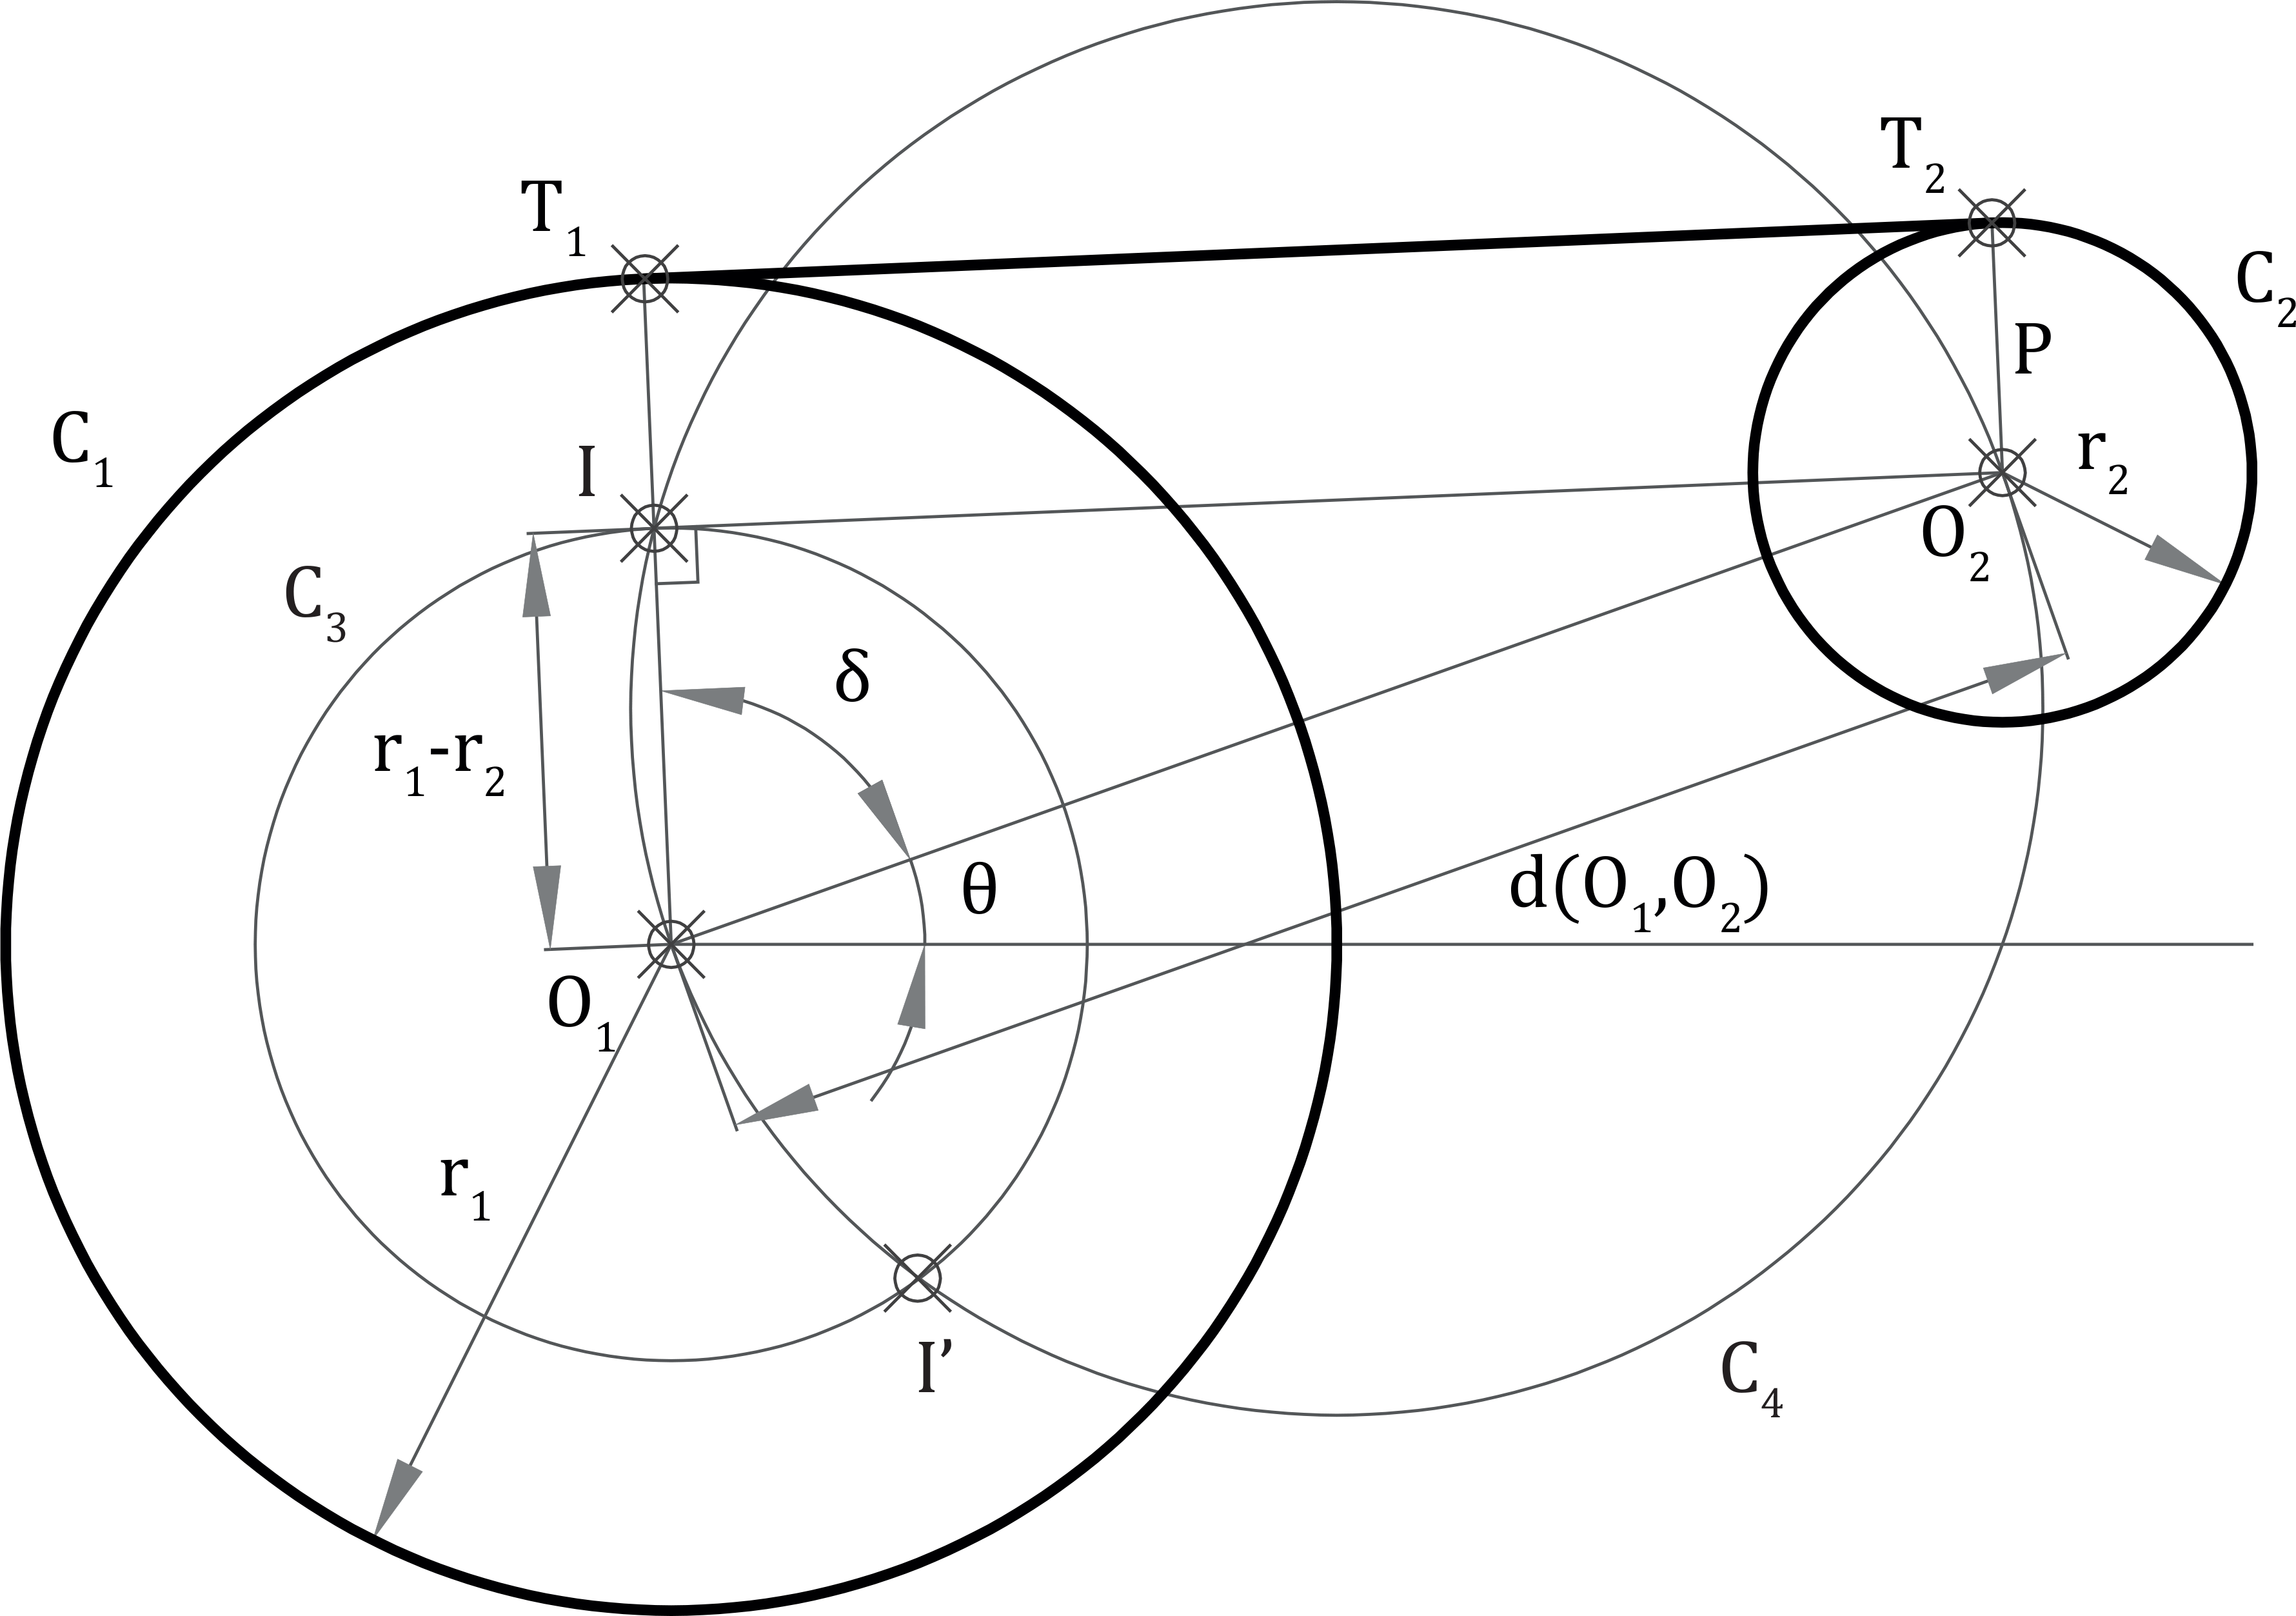
\includegraphics[height=7cm]{fig/rtrapezoid-solution}
  \caption[Rounded trapezoid problem solution]{Both analytic and constructive
    solutions to the rounded trapezoid problem.}%
  \label{fig:eval.studies.rtrapezoid.sol}
\end{figure}

\begin{enumerate}
  \item $C_3 = \mathrm{circle}\left(O_1, r_1 - r_2\right)$
  \item $M = \mathrm{midpoint}\left(O_1, O_2\right)$
  \item $d = \mathrm{length}\left(\overline{O_1 O_2}\right)$
  \item $C_4 = \mathrm{circle}\left(M, \frac{d}{2}\right)$
  \item $I,I' = \mathrm{intersection}\left(C_3, C_4\right)$
  \item $P = \mathrm{parallel}\left(\overline{IO_1, O_2}\right)$
  \item $T_1 = \mathrm{intersection}\left(IO_1, C_1\right)$
  \item $T_2 = \mathrm{intersection}\left(P, C_2\right)$
\end{enumerate}

Despite the adequacy of the \textit{analytic solution} for the design problem at
hand, it only produces the external tangent needed to solve this specific
problem, which works well if the circle's center is on the 1\textsuperscript{st}
and 2\textsuperscript{nd} quadrants: however, in the remaining quadrants, it
produces an unintended tangent.  In contrast, our \textit{constructive approach}
is capable of producing a solution independently of how the circles are
arranged.

The advantage of using well-established functions from \ac{CGAL} is that they
deal with degenerate cases better than re-implementations of the same
functionality from scratch.  For instance, in the case of concentric circles,
the intersection between those circles does not produce an error; instead, it
produces an empty result.  In the case of the proposed \textit{analytic
solution}, the distance between the circles' centers is zero, which leads to a
division-by-zero error.

Architects and designers are used to manipulating \acp{GC}, such as
\textit{tangency}, \textit{parallelism}, and \textit{intersection}, and less
inclined to deal with the mathematical intricacies of analytic geometry, which
makes the second approach more appealing to them.  To that end, we can introduce
the $\mathrm{tangent_{lines}}$ functionality, which, given two circles $C_1$ and
$C_2$, produces a sequence of tangent lines between the circles, allowing the
user to select the lines that best suit the problem.  This allows us to reduce
the solution to the single step
\begin{itemize}
  \item[] $\overline{T_1 T_2},\ldots = \mathrm{tangent_{lines}}\left(C_1,
  C_2\right)$
\end{itemize}
where $\overline{T_1 T_2}$ is one of the lines of the sequence.

Depending on how the circles are arranged, there can be multiple solutions:
\begin{enumerate*}[label= (\arabic*)]
  \item no segments, if one circle contains the other,
  \item two segments, if the circles intersect, or
  \item four segments, if the circles are disjoint.
\end{enumerate*}
The advantage of having the $\mathrm{tangent_{lines}}$ functionality is that it
is capable of finding every solution to the generic \textit{tangent line to two
circles} problem.  Hence, the user can reutilize this functionality each time
a different problem of a similar nature arises.

\subsection{Star with Semicircles}%
\label{sec:eval.studies.star}

The third case study is a star shape with semicircles.  This shape was inspired
by César Pelli's Petronas tower floor plan, which in turn mimics Islamic
patterns.  The contour of the Petronas tower floo plan is formed by two
overlapping congruent squares, forming an octagram known as Star of Lakshmi, and
by eight circles centered on each of the eight intersection points and tangent
to the bounding octagon.  This shape can be generalized to a parametric shape
defined by three parameters: origin $O$, radius $r$, and number of vertices $n$
(\cref{fig:eval.studies.star.prob.params}).  Note that the number of vertices
cannot be less than five.  Five variations, comprising stars with 5 to 9
vertices, are illustrated in \cref{fig:eval.studies.star.prob}.

\begin{figure}[htb]
  \centering
  \subcaptionbox{\label{fig:eval.studies.star.prob.params}%
    Star parametrization: origin $O$, radius $r$, and number of vertices $n$.}
    {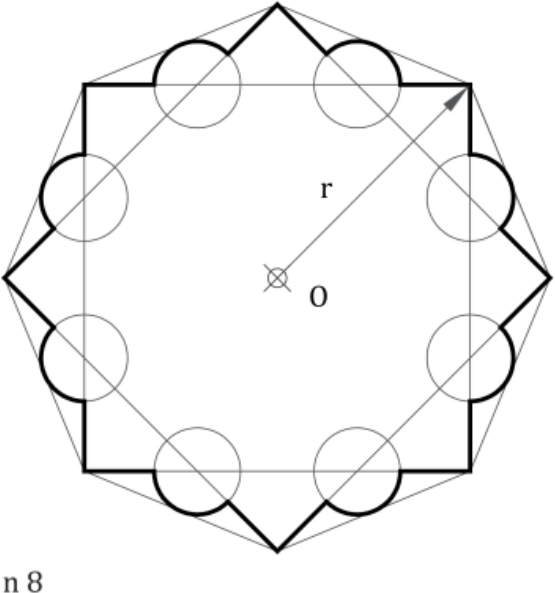
\includegraphics[height=7cm]{fig/star-problem-params}}
  \hfill
  \subcaptionbox{\label{fig:eval.studies.star.prob.vars}%
    Star shape variations: variations change the values of the number of
    vertices $n$.}
    {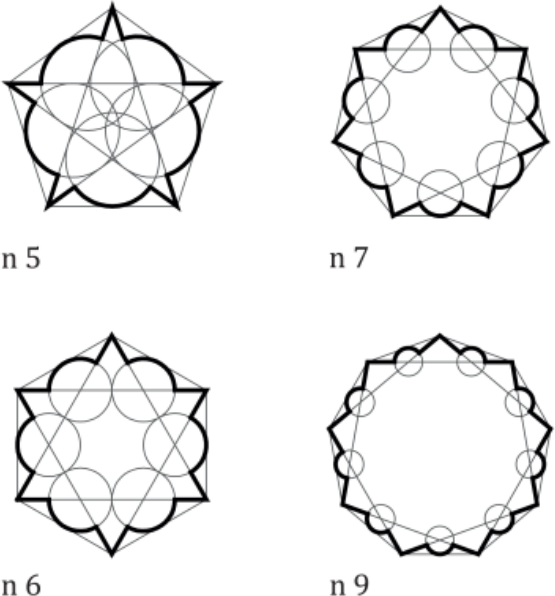
\includegraphics[height=7cm]{fig/star-problem-vars}}
  \caption[Star with semicircles problem]{Star with semicircles problem:
    \subref{fig:eval.studies.star.prob.params} shows our parametrization of
    the star which can be used to generate shape variations, some of them
    shown in \subref{fig:eval.studies.star.prob.vars}.}%
  \label{fig:eval.studies.star.prob}
\end{figure}

Both analytic and constructive solutions are based on computing one side of the
star, composed of the line segment $\overline{V_1 I_1}$, the arc centered on
$O_1$ from $I_1$ to $I_2$, with radius $r_1$, and the line segment 
$\overline{I_2 V_2}$ (\cref{fig:eval.studies.star.sol}).  The remaining sides
result from the recursive application of the preceding side with a rotation
transformation around the center.

\begin{figure}[htb]
  \centering
  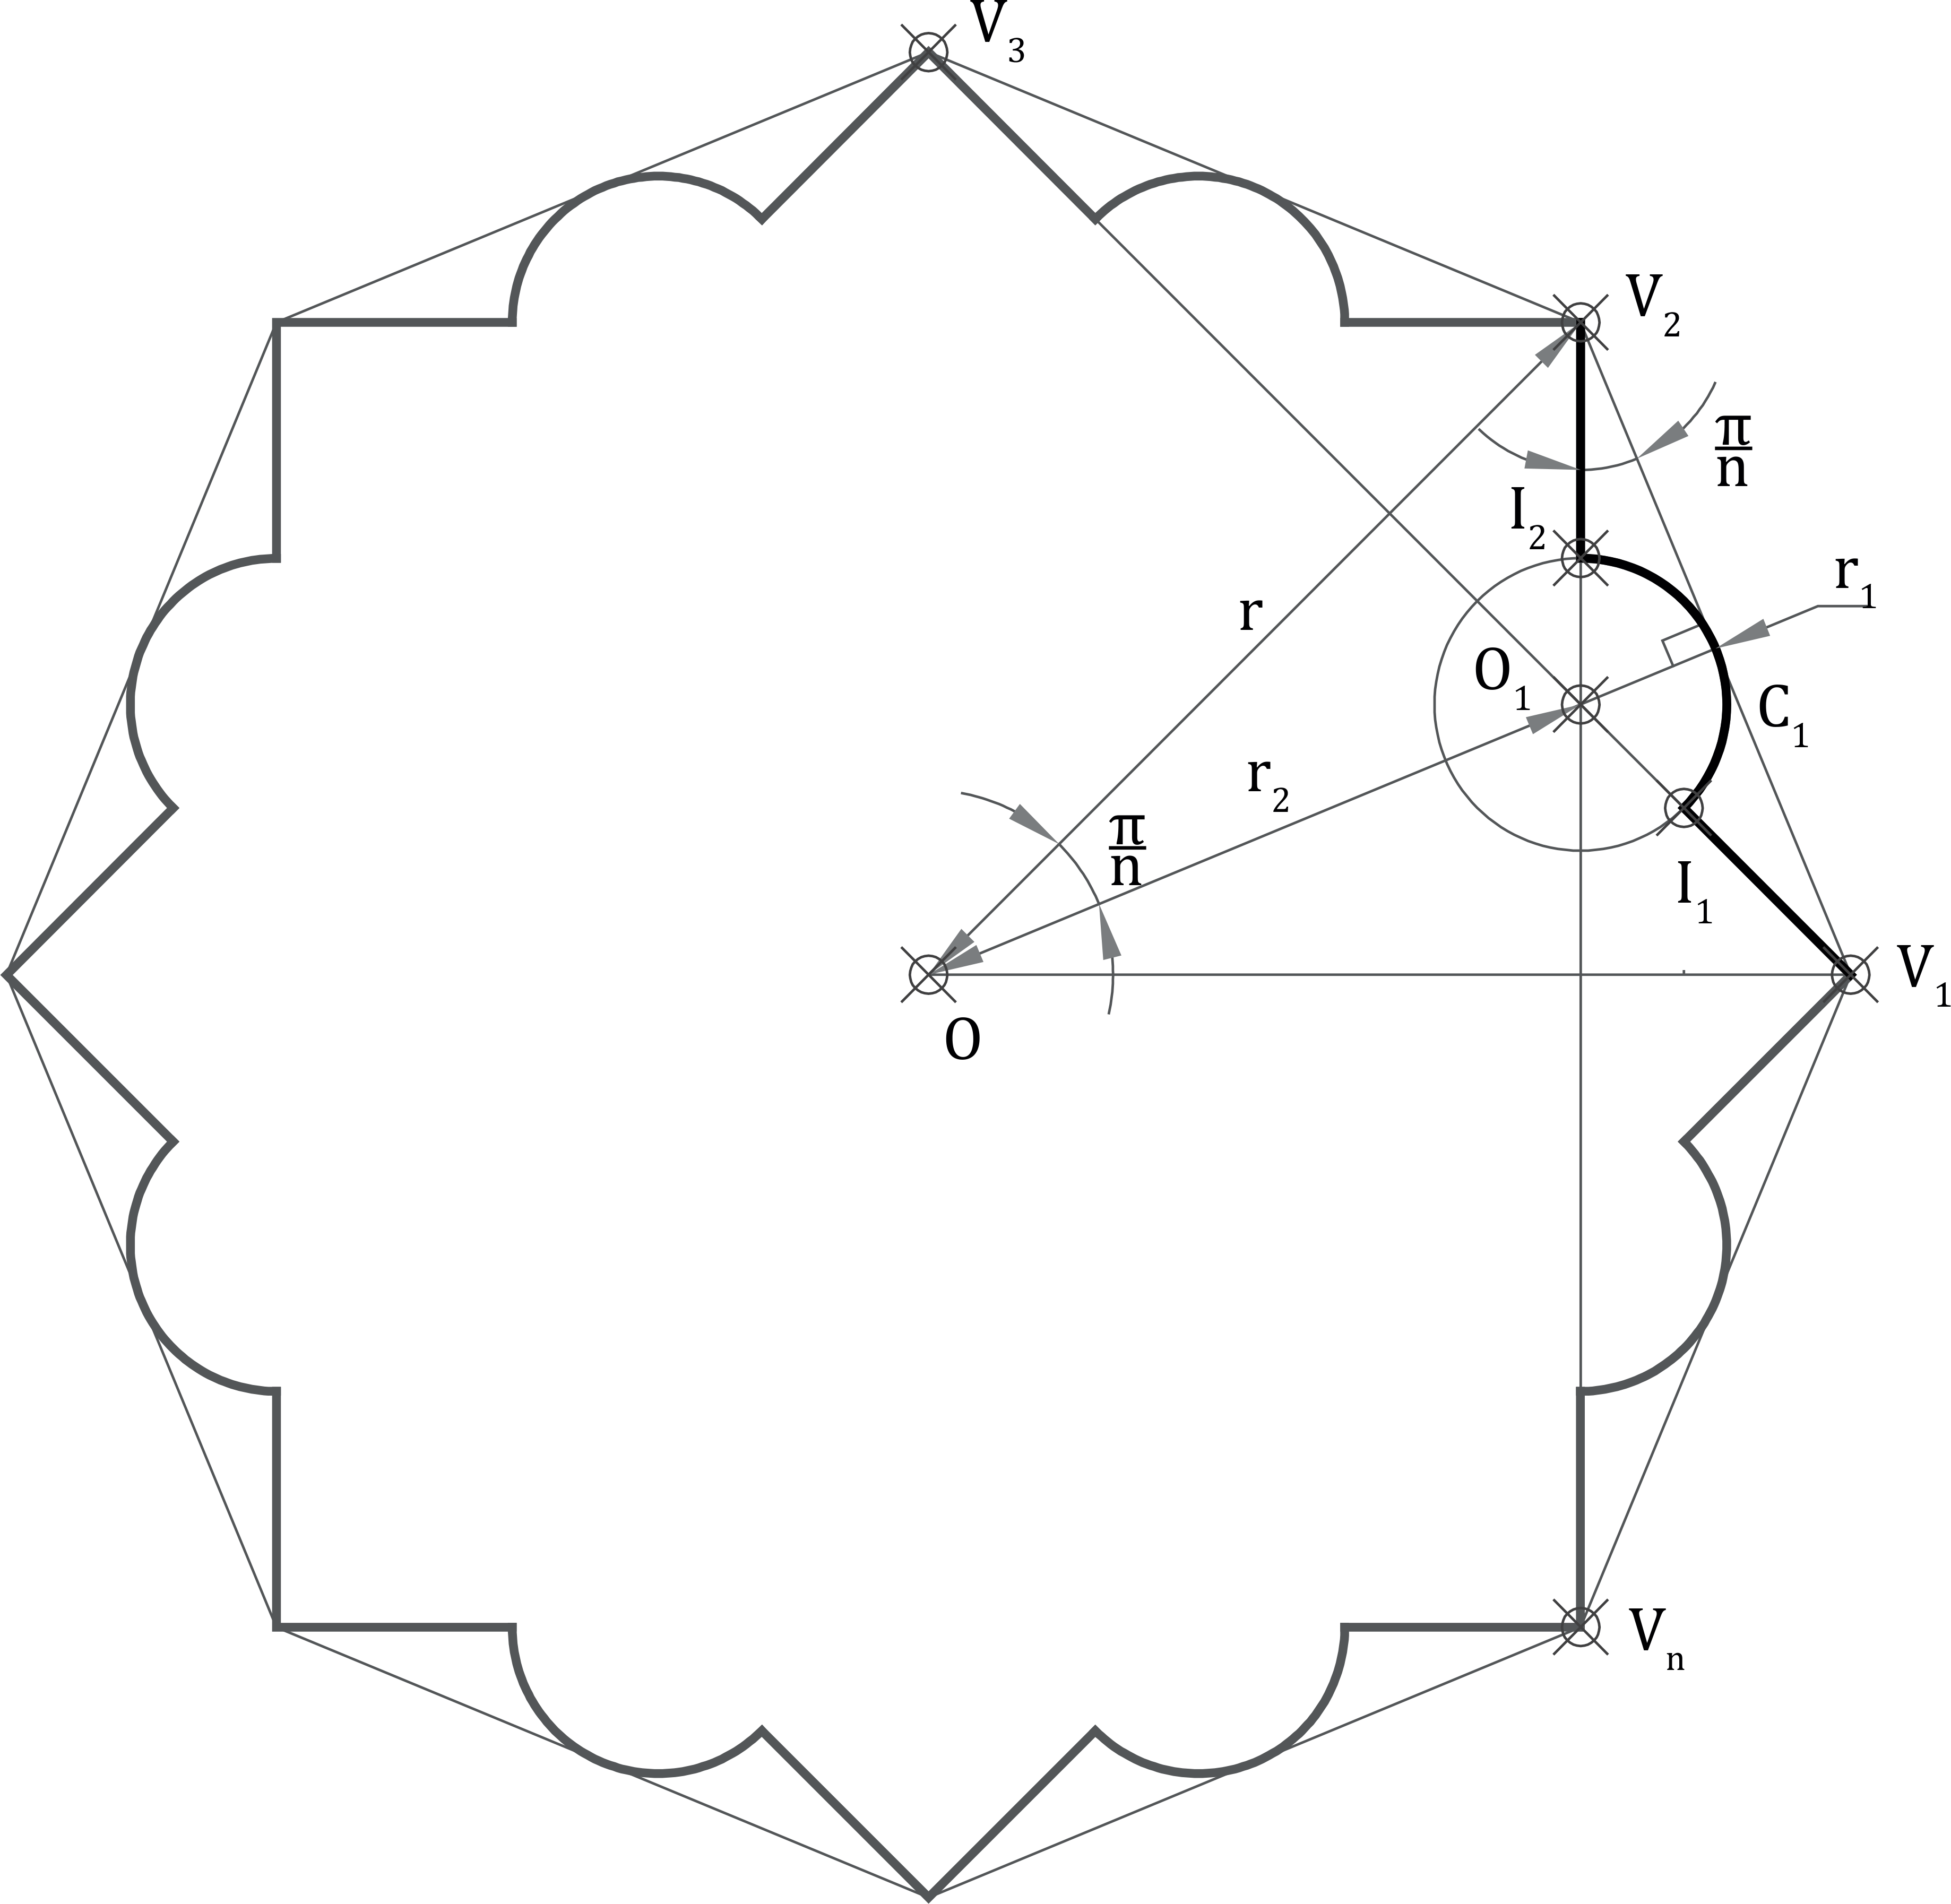
\includegraphics[height=9cm]{fig/star-solution}
  \caption[Star with semicircles problem solution]{ Both analytic and
    construction solutions to the star with semicircles problem.}%
  \label{fig:eval.studies.star.sol}
\end{figure}

The \textit{analytic solution} is described below.  The radius $r_1$ of the
circle $C_1$ is calculated by step \ref{enum:eval.studies.star.r1}, the radius
$r_2$ is defined by step \ref{enum:eval.studies.star.r2}, and its center $O_1$
is given by step \ref{enum:eval.studies.star.O1}.  The intersection points $I_1$
and $I_2$ are given by a rotation around $O_1$
(\cref{fig:eval.studies.star.sol}).

\begin{enumerate}
  \item $r_1 = r\frac{\sin^2\frac{\pi}{n}}{\cos\frac{\pi}{n}}$%
  \label{enum:eval.studies.star.r1}
  \item $r_2 = r\cos\frac{\pi}{n} - r_1$%
  \label{enum:eval.studies.star.r2}
  \item $O_1 = O + \left(r_2, \angle\frac{\pi}{n}\right)$%
  \label{enum:eval.studies.star.O1}
  \item $I_1 = O_1 + \left(r_1, \angle\frac{2\pi}{n} - \frac{\pi}{2}\right)$
  \item $I_2 = O_1 + \left(r_1, \angle\frac{\pi}{2}\right)$
\end{enumerate}

The \textit{construction solution} is based on finding the position and size of
the circle $C_1$ (see \cref{fig:eval.studies.star.sol}).  Two \ac{GC}
primitives were employed in this solution, namely \textit{intersection}, and
\textit{tangent circle to one line}.

\begin{enumerate}
  \item $O_1 = \mathrm{intersection}\left(\overline{V_1 V_3}, \overline{V_2
  V_n}\right)$
  \item $C_1 = \mathrm{tangent_{circle}}\left(O_1, \overline{V_1 V_2}\right)$
  \item $P,r_1 = C_1$
  \item $I_1 = \mathrm{intersection}\left(\overline{V_1 V_3}, C_1\right)$
  \item $I_2 = \mathrm{intersection}\left(\overline{V_2 V_n}, C_1\right)$
\end{enumerate}

As seen in the other cases, the constructive solution is more understandable, as
one can easily reproduce it step-by-step by hand, using a ruler and a compass.

\subsection{Voronoi Diagram}%
\label{sec:eval.studies.voronoi}

Our fourth case study is that of Voronoi diagrams, which are used in a variety
of design fields.  For instance, several facade designs exhibit a Voronoi
appearance, such as PTW Architects' Beijing National Aquatics Center,
ARM\footnote{\url{https://armarchitecture.com.au/projects/melbourne-recital-centre/}.
Not to be mistaken with the ARM family of computing architectures for computer
processors.} Architecture's Melbourne Recital Centre, and Hassell's Alibaba
Headquarters.

In its simplest version, a Voronoi diagram consists of partitioning a plane into
regions from a set of points, called \textit{sites}; for every site, each region
contains every point in the plane closer to that site than to any other site.
The sites are typically randomly distributed points, although they can follow
other distributions.  \Cref{fig:eval.studies.voronoi.prob} shows three Voronoi
diagrams generated from entirely randomly distributed points
(\cref{fig:eval.studies.voronoi.prob.rand}), from random points with one
attractor point in the bottom-left corner
(\cref{fig:eval.studies.voronoi.prob.1attr}), and from random points with one
attractor line at the bottom edge (\cref{fig:eval.studies.voronoi.prob.edge}).
An attractor object is responsible for controlling the density of random points
based on the distance to it.

\begin{figure}[htb]
  \subcaptionbox{\label{fig:eval.studies.voronoi.prob.rand}%
    Randomly distributed points.}
    {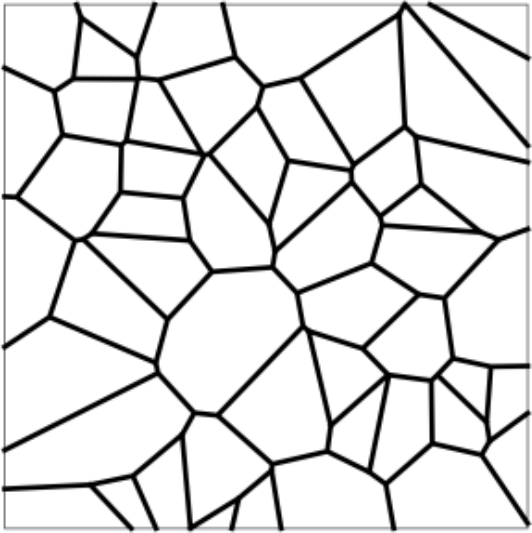
\includegraphics[height=5cm]{fig/voronoi-problem-rand}}
  \hfill
  \subcaptionbox{\label{fig:eval.studies.voronoi.prob.1attr}%
    Randomly distributed points with one attractor point in the bottom-left.}
    {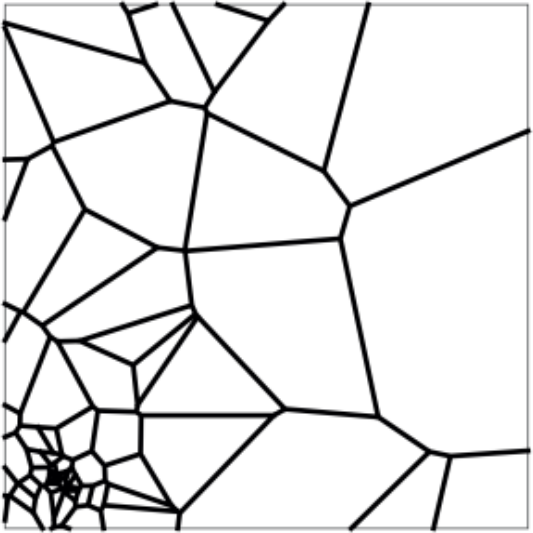
\includegraphics[height=5cm]{fig/voronoi-problem-1attr}}
  \hfill
  \subcaptionbox{\label{fig:eval.studies.voronoi.prob.edge}%
    Randomly distributed points with an attractor line at the bottom.}
    {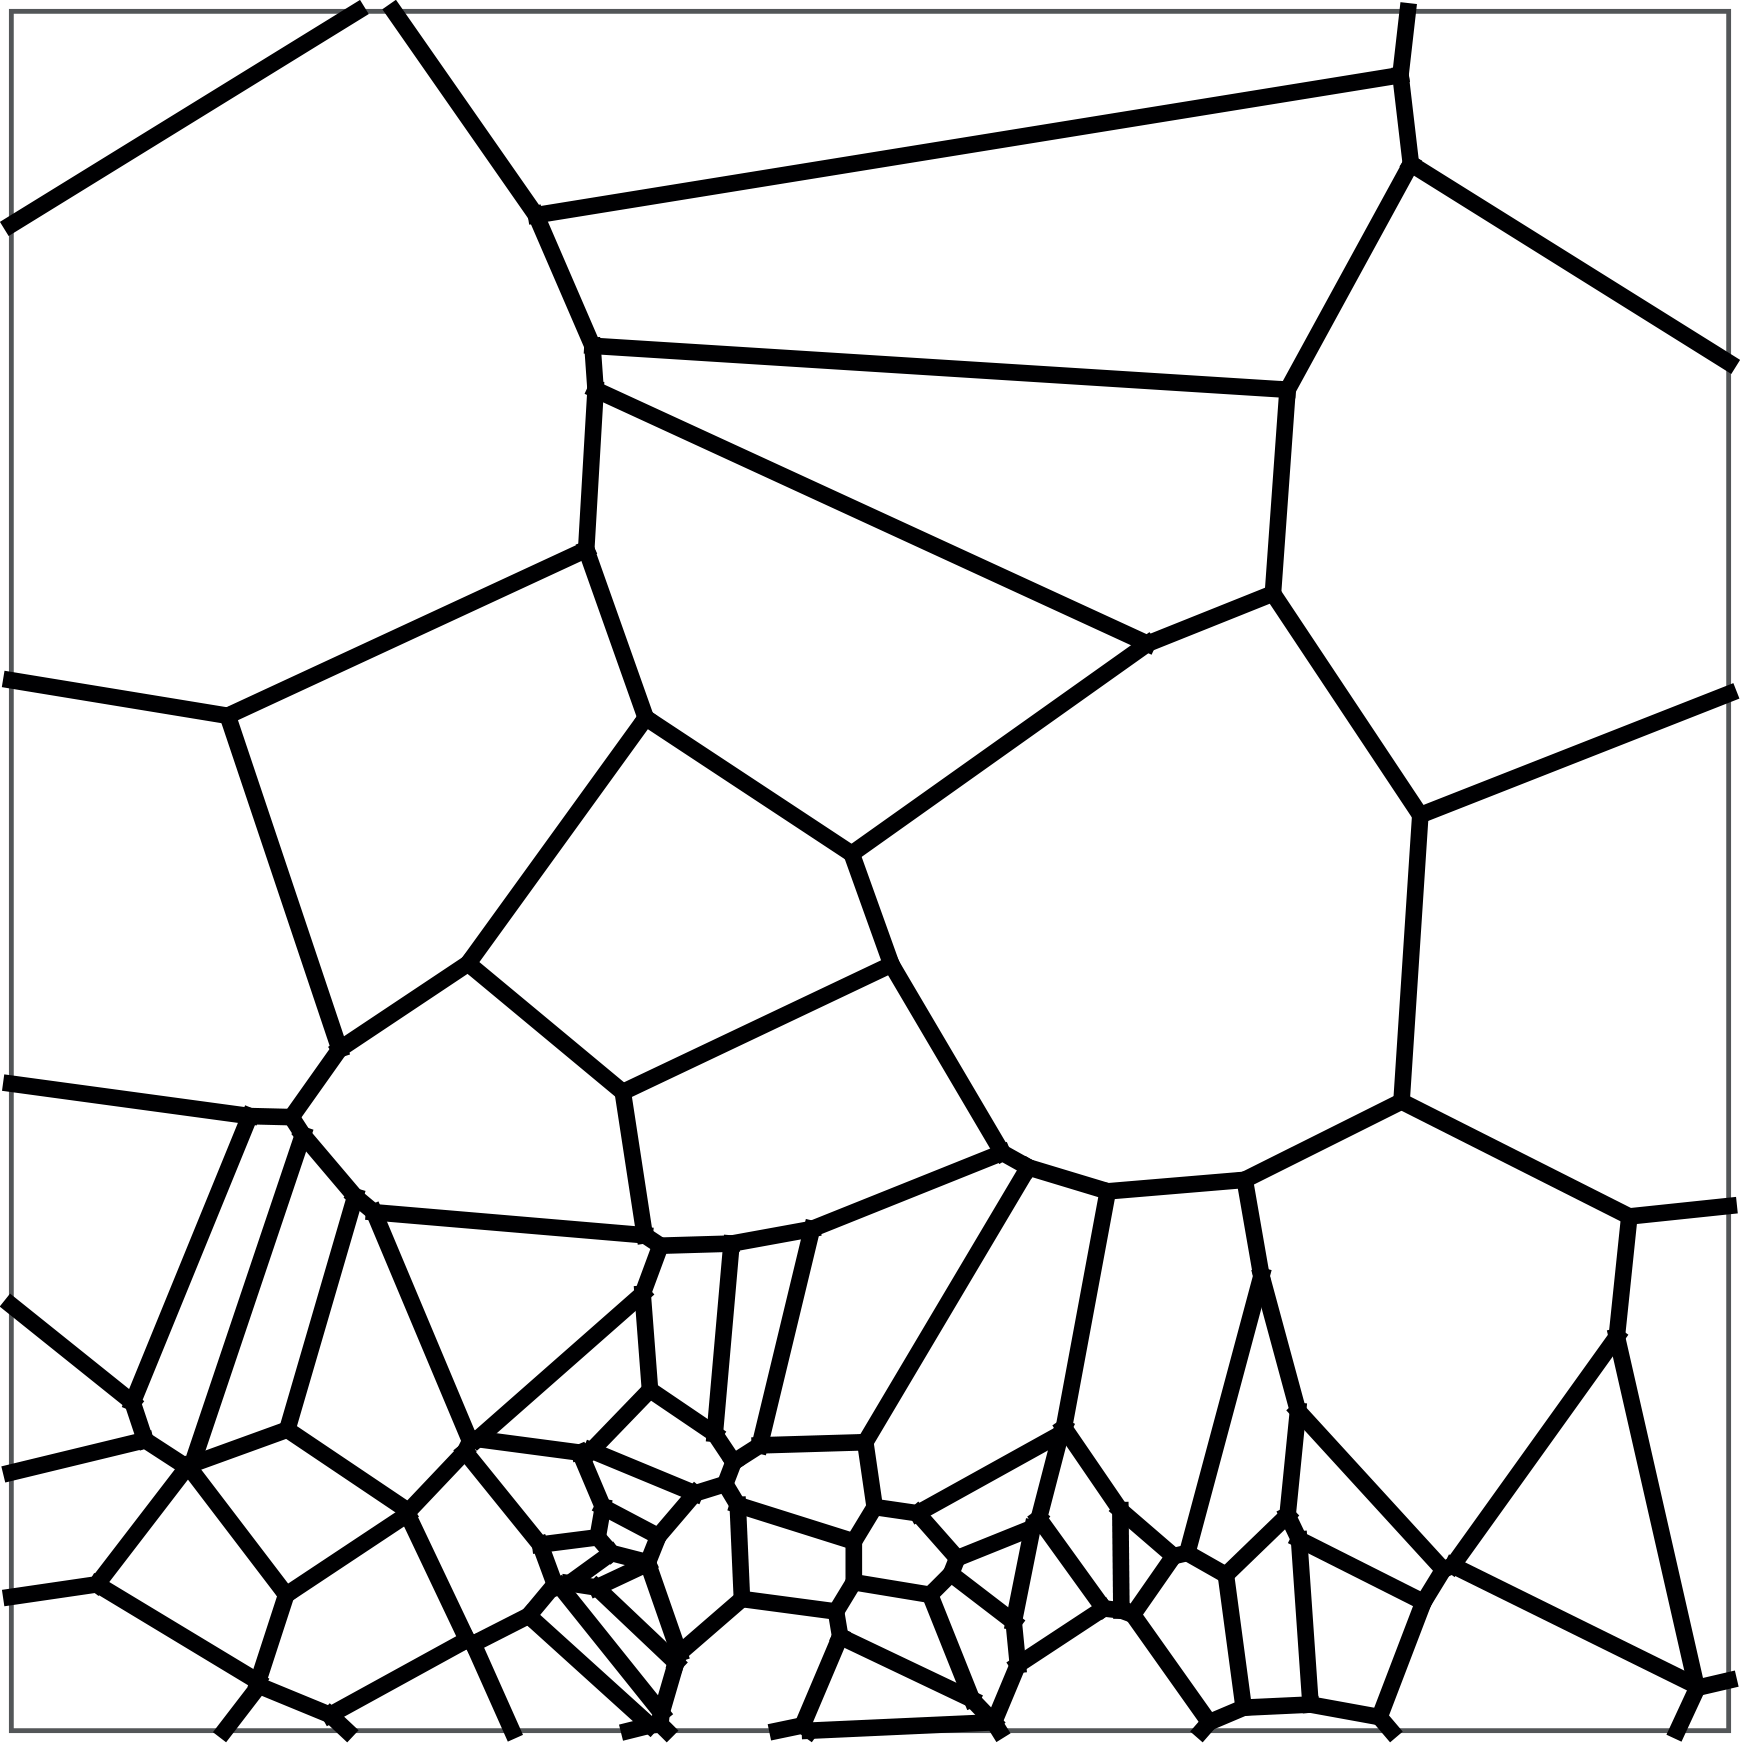
\includegraphics[height=5cm]{fig/voronoi-problem-edge}}
  \caption[Voronoi diagram problem]{
    Voronoi diagram problem: depicted are three Voronoi diagrams variations
    which are mostly generated at random.
    \subref{fig:eval.studies.voronoi.prob.rand} is entirely random,
    \subref{fig:eval.studies.voronoi.prob.1attr} expands on the latter with an
    attractor point, and \subref{fig:eval.studies.voronoi.prob.edge} goes even
    further by using an entire attractor line.}%
  \label{fig:eval.studies.voronoi.prob}
\end{figure}

Both the analytic and constructive methods focus on computation of a vertex
relies on the computation of the \textit{circumcenter} of a triangle, for
instance, triangle $\triangle P_1 P_2 P_3$
(\cref{fig:eval.studies.voronoi.sol}).

\begin{figure}[htb]
  \centering
  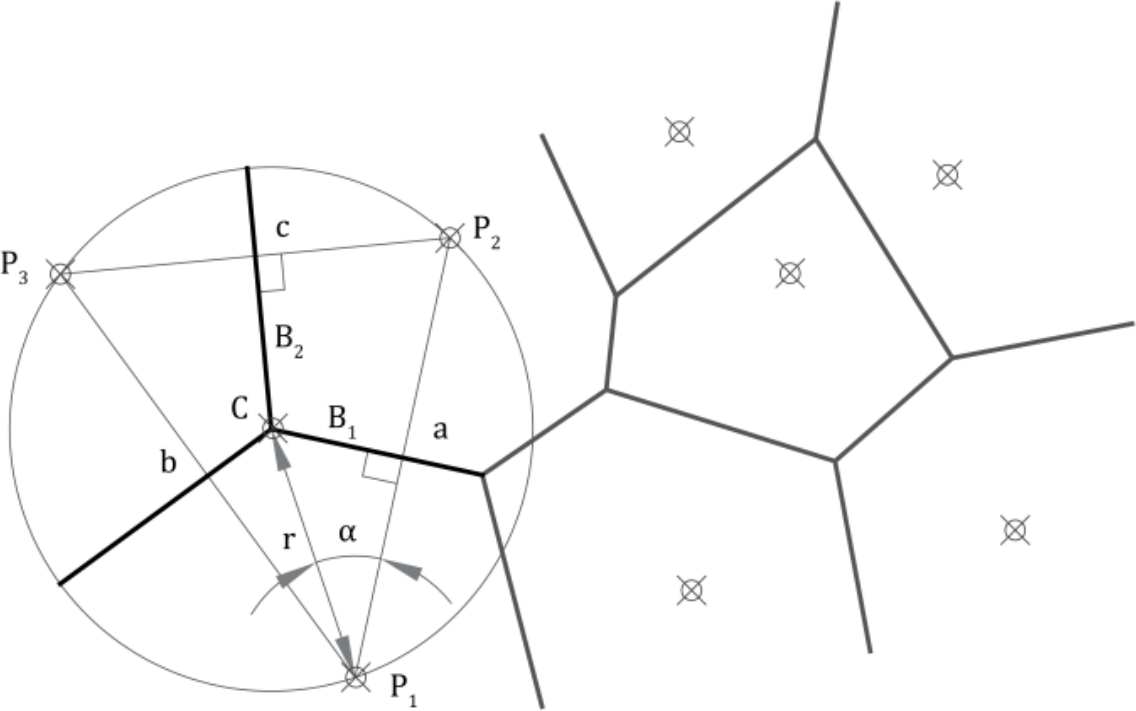
\includegraphics[height=6cm]{fig/voronoi-solution}
  \caption[Voronoi problem partial solution]{
    Analytic and constructive approaches to computing a Voronoi vertex via
    computing the circumcenter of every triangle in the Delaunay triangulation
    whose vertices are the Voronoi diagram's sites.}%
  \label{fig:eval.studies.voronoi.sol}
\end{figure}

There are several possible \textit{analytic solution} to compute a triangle's
circumcenter.  One of them is based on the \textit{circumradius} formula (step
\ref{enum:eval.studies.voronoi.sol.a.circum}), where $a$, $b$, and $c$ are the
lengths of the triangle's sides (step
\ref{enum:eval.studies.voronoi.sol.a.tri}) and $A$ is the triangle's area (step
\ref{enum:eval.studies.voronoi.sol.a.area}).  The circumcenter $C$ can then be
easily computed by a translation (step
\ref{enum:eval.studies.voronoi.sol.a.move}) from $P_1$ following the angle
$\alpha$ (step \ref{enum:eval.studies.voronoi.sol.a.alpha}).

\begin{enumerate}
  \item $a, b, c = \lVert P_2 - P_1 \rVert, \lVert P_3 - P_1 \rVert, \lVert P_3
  - P_2 \rVert$%
  \label{enum:eval.studies.voronoi.sol.a.tri}
  \item $s = \frac{a + b + c}{2}$
  \item $A = \sqrt{s(s - a)(s - b)(s - c)}$%
  \label{enum:eval.studies.voronoi.sol.a.area}
  \item $r = \frac{abc}{4A}$%
  \label{enum:eval.studies.voronoi.sol.a.circum}
  \item $\alpha = \arccos\frac{a}{2r}$%
  \label{enum:eval.studies.voronoi.sol.a.alpha}
  \item $C = P_1 + \left(r, \angle\alpha\right)$%
  \label{enum:eval.studies.voronoi.sol.a.move}
\end{enumerate}

The \textit{constructive solution} computes the circumcenter, given by the
intersection of the edges' perpendicular bisectors.  In fact, this has been
exemplified in \cref{chap:intro}.  Two \ac{GC} primitives were employed in this
solution, namely \textit{bisector} and \textit{intersection}.

\begin{enumerate}
  \item $B_1 = \mathrm{bisector}\left(\overline{P_1 P_2}\right)$
  \item $B_2 = \mathrm{bisector}\left(\overline{P_2 P_3}\right)$
  \item $C = \mathrm{intersection}\left(B_1, B_2\right)$
\end{enumerate}

We can increase the abstraction level of the solution by using the
\textit{circumcenter} functionality implemented in our solution, which, in
reality, is implemented in \ac{CGAL}:

\begin{enumerate}
  \item $C = \mathrm{circumcenter}\left(P_1, P_2, P_3\right)$
\end{enumerate}

The circumcenter problem is only a small part of the generation of a Voronoi
diagram, since we first need to build a Delaunay triangulation.  We can then 
apply the $\mathrm{circumcenter}$ functionality to find the Voronoi vertices and
draw the diagram's edges.  This set of steps can be abstracted away in a
functionality called \textit{voronoi} that, given a set of points $P_S$,
produces a 2D Euclidean Voronoi diagram:

\begin{enumerate}
  \item $V = \mathrm{voronoi}\left(P_S\right)$
\end{enumerate}

Implementing this functionality from scratch is a demanding and error-prone
task.  Fortunately, \ac{CGAL} already has an algorithm that produces robust 2D
Euclidean Voronoi diagrams that can handle degenerate cases, such as dealing
with three or more collinear points.  This algorithm, much like the
\textit{circumcenter} functionality, was entirely repurposed, and made available
in \texttt{CGAL.jl}, and, thus, it is also available in our solution.
